\documentclass[14pt]{article}

\usepackage[a4paper]{geometry}
\geometry{ hmargin=2.5cm, vmargin=1.5cm }

\usepackage{attachfile}
\usepackage{graphicx}
\usepackage{amsmath}
\usepackage{placeins}
\usepackage{color}
\usepackage{alltt}

\usepackage[]{algorithm2e}
\usepackage{amssymb}
\usepackage{ulem}
\usepackage{subfig}
\usepackage{float}
\usepackage[french]{babel}
\usepackage[T1]{fontenc}  
\usepackage[utf8]{inputenc}
\usepackage{minted}
\usepackage{tcolorbox}
\usepackage{etoolbox}
\BeforeBeginEnvironment{minted}%
     {\begin{tcolorbox}}%
\AfterEndEnvironment{minted}
   {\end{tcolorbox}}%
\BeforeBeginEnvironment{inputminted}%
     {\begin{tcolorbox}}%
\AfterEndEnvironment{inputminted}
   {\end{tcolorbox}}%

\let\oldinputminted\inputminted
\renewcommand{\inputminted}[2]{\begin{tcolorbox}\oldinputminted[breaklines]{#1}{#2}\end{tcolorbox}}

\renewcommand{\thesection}{\Roman{section}}
\renewcommand{\thesubsection}{\thesection .\arabic{subsection}}


\setcounter{lofdepth}{1}
\setcounter{secnumdepth}{4}





\title{Solution challenge SSTIC 2016}
\author{Benoit Maurin}
\begin{document}
\date{}

\maketitle

\tableofcontents

\section*{Résumé}
Avertissement: désolé si ya des phrases qui n'ont pas de sens, il me reste 10 minutes pour pas dépasser la deadline :).
Oups, +2. Le système d'ouverture des pièces jointes fonctionne pas top chez moi.
Considérez utiliser:
\begin{minted}{bash}
$ pdftk report.pdf unpack_files 
$ #
\end{minted}

On commence avec un fichier de capture réseau. Le flux contenu est un téléchargement d'un zip par HTTP.
Ce zip contient un serveur web avec un jeu.

\section{Récupération du jeu}

Sur le site il nous est donné un ficher \url{http://static.sstic.org/challenge2016/challenge.pcap}.
On l'ouvre avec Wireshark et on observe du trafic HTTP où un fichier zip est téléchargé.
Pour obtenir le zip, clique droit sur un paquet > Follow > TCP Stream > Save as.
En enlevant les headers HTTP du fichier sauvegardé l'archive peut être extraite.

\inputminted{bash}{./sessions/recover_game.txt}

Un navigateur web et c'est parti.


\section{Niveau 1}

Trois challenges possibles pour ce niveau.
\begin{itemize}
\item[SOS-Fant0me.zip] Capture réseau du trojan GhOst RAT
\item[calc.zip] Programme de calculatrice TI-83+
\item[radio.zip] Samples SDR d'une session GSM?
\end{itemize}

\FloatBarrier
\subsection{SOS}

\subsubsection{En deux mots}
 Décoder Gh0st RAT traffic en utilisant chopshop.

\subsubsection{En trois}

Wireshark à nouveau. Les données TCP sont préfixée par {\em Gh0st}. Avec l'aide du net, on se doute rapidement que c'est une session du trojan Gh0st RAT. Pour décoder le trafic \url{https://github.com/MITRECND/chopshop/blob/master/modules/gh0st_decode.py}.


\begin{minted}[breaklines]{bash}
$ chopshop --savedir=tmp/ -f SOS-Fant0me.pcap "gh0st_decode --savefiles"
$ unzip 'C__Users_sstic_Documents_Challenge SSTIC 2016_Stage 1_sstic2016-stage1-solution.zip'
$ cat solution.txt
368BE8C1CC7CC70C2245030934301C15
# $
\end{minted}

\begin{minted}{text}
Clé: 368BE8C1CC7CC70C2245030934301C15
\end{minted}

\FloatBarrier
\subsection{Calc}

\subsubsection{TL;DR}
TI83+ instructions vers C++ pour bruteforce input.

\subsubsection{J'annonce, cette partie est chiante}

\begin{minted}{bash}
$ file SSTIC16.8xp
SSTIC16.8xp: TI-83+ Graphing Calculator (program)
$
\end{minted}

Dans l'émulateur \url{http://lpg.ticalc.org/prj_tilem/}, clique droit > Send file, puis choisir SSTIC16.8xp.
Ensuite il faut cliquer sur les boutons PRGM > 1 > Enter. Le programme nous demande un chiffre. Au bout d'un certain temps après en avoir rentré un, s'affiche WHP le message {\em PERDU}.
Le challenge est de trouver le bon numéro. Il est possible de regarder les sources du programmes en cliquant PRGM > Flèche Droite (Menu Edit) > 1 > Enter. Mais bon, c'est vraiment pas pratique de lire le code comme çà. Il est possible de convertir le fichier 8xp en instructions texte à \url{http://ti.zewaren.net/fr/83p--txt-converter.php}.

En jetant un oeil aux instructions, on trouve:
\begin{minted}{text}
Lbl 19
ClrHome
If A=3298472535:Then
Z->rand
21->S
1->X
4->Y
Output(3,7,"KEY:")
Goto 21
Else
Output(3,6,"PERDU")
End
Goto X
\end{minted}

On connaît maintenant la condition de succès. Malheureusement la clé affichée n'est pas hardcodée dans les instructions mais décodée au cours du programme.
Au début du programme on observe aussi:

\begin{minted}{text}
Lbl 2
" "->Str1
Repeat not(A
A/2->A
sub("01",1+not(not(fPart(Ans))),1)+Str1->Str1
iPart(A->A
End
sub(Str1,1,length(Str1)-1)->Str1
While length(Str1)<32
"0"+Str1->Str1
End
Goto 0
\end{minted}

Cette fonction donne la représentation binaire d'un nombre et ajuste la chaine de caractère pour qu'elle soit de taille au moins 32.
On en déduit que le nombre attendu soit représentable sur 32 bits. Çà ouvre la voix du bruteforce.
J'ai jamais écrit de programme ti83+ et aussi le programme s'exécute sur plusieurs seconds. Pas d'approche black box donc :(.
J'ai pas trouvé de compilateur vers x86 des instructions TI (peu cherché aussi), alors il va falloir transcrire le programme dans un autre langage (ici C++).
Les instructions annotées sont visible dans ce
\textattachfile[mimetype=text/plain,color=0 0 0.5]{challs/calc/tsf.txt}{fichier}.
Une fois annoté, il n'est pas difficile de trouver le code équivalent.

\begin{minted}{cpp}
// Bruteforcing of the key.
u32 tb[] = {
  0,          1996959894, 3993919788, 2567524794, 124634137,  1886057615,
  3915621685, 2657392035, 249268274,  2044508324, 3772115230, 2547177864,
..
/* Edited for display*/
};

const u32 resv = 3298472535;

u32 proc(u32 a) {

  u32 c0 = 4294967295;
  REP (n, 4) {
    u32 ax = a >> (n * 8) & 0xff;
    u32 cx = ax ^ (c0 & 0xff);
    c0 = c0 >> 8;
    c0 = tb[cx] ^ c0;
  }
  c0 = ~c0;
  return c0;
}

int main() {
  for (u32 i = 0;; ++i) {
    u32 res = proc(i);
    if (res == resv) {
      printf("found at %u\n", i);
      break;
    }
    // res: c49ab257

    if ((i + 1) == 0)
      break;
    // found at 89594902
    // 57D9F82b49c1eb3993cb82d26e37f69c
  }

  return 0;
}
\end{minted}

Le fichier complet est disponible dans la section ressources.

Le nombre à rentrer est {\em 89594902}.
\begin{figure}[H]
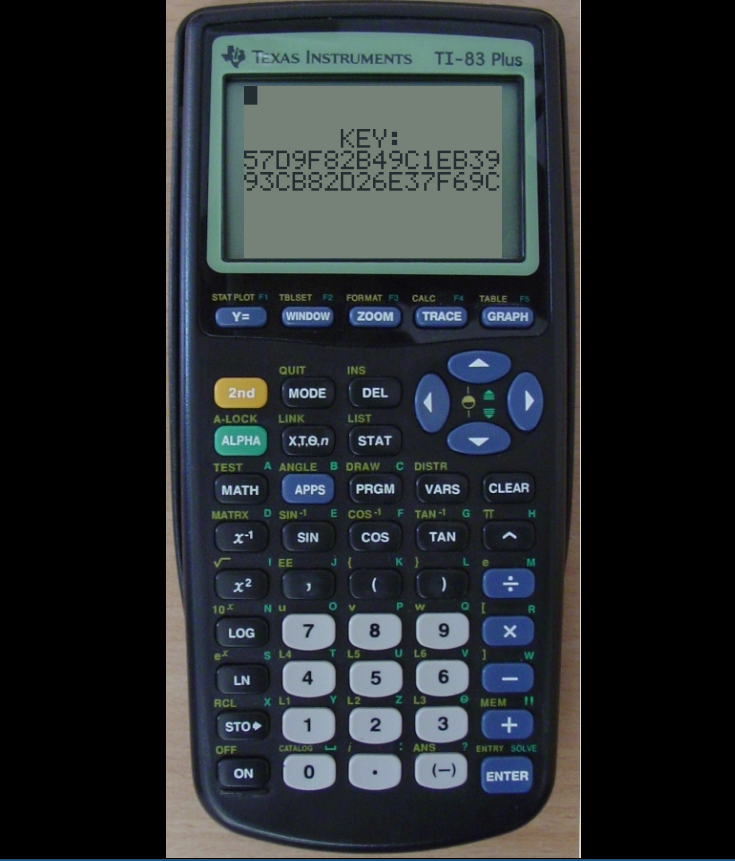
\includegraphics[width=0.8\textwidth]{./challs/calc/snapshot1.png}
\centering
\end{figure}

En rentrant ce nombre dans l'émulateur, on obtient: 
\begin{minted}{text}
57D9F82b49c1eb3993cb82d26e37f69c
\end{minted}

\subsubsection{Ressources}
\begin{itemize}
\item \textattachfile[mimetype=text/plain,color=0 0 0.5]{challs/calc/tsf.txt}{instructions annotées}
\item \textattachfile[mimetype=text/plain,color=0 0 0.5]{challs/calc/solve.cpp}{solve.cpp}
\end{itemize}

\FloatBarrier
\section{Niveau 2}
Après avoir rentré les clés trouvées en parlant au garde (d'ailleurs impossible de faire copier coller, injouable!), on débloque d'autres challenges.
\begin{itemize}
\item[efi] Une application EFI.
\item[huge] Une tar bomb contenant un elf.
\item[loader] Un exe (j'en sais pas plus :) .)
\end{itemize}

À ce moment là j'avais que mon portable avec 4Go de RAM. C'est pas une expérience plaisante de lancer une VM windows dans ces conditions. En plus je connais très peu Windows (à mon futur regret), donc efi et huge ce sera.


\FloatBarrier
\subsection{efi}
\subsubsection{La version où je raconte pas ma vie}
Patch du binaire pour bruteforcer char par char. Automatisation du tout avec communication pty qemu + génération de script efi.

\subsubsection{Par contre là...}
Pour une introduction sur EFI, je vous renvoie sur \url{https://en.wikipedia.org/wiki/Unified_Extensible_Firmware_Interface}. Cette page en connaît plus que moi.

Première étape, faire tourner le programme. J'ai encore que mon portable et j'ai pas envie de ruiner mon installation trifouillant dans le BIOS. QEMU est une solution plus sûre.
On trouve des infos sur \url{http://www.tianocore.org/ovmf/}

\begin{minted}{bash}
$ unzip OVMF-X64-r15214.zip 
$ mkdir hda-contents
$ cp foo.efi ./hda-contents
$ qemu-system-x86_64 -L . -hda fat:hda-contents -bios OVMF.fd
  # trying to boot on the network, mkay
  Shell > fs0:
  FS0:\> f00.efi aaaaaaaaaaaaaaaaaaaaaaaaaaaaaaaa 
  UEFI checker
  Sorry :(
\end{minted}

L'application s'attend à une chaine hexa de 32 caractères. Ce sera probablement la clé du niveau.

IDA peut ouvrir des applis EFI, fantastique. 
Pas de symboles externes, les fonctions de l'équivalent libc sont accessibles par les arguments du main.
Çà ressemble à:
\begin{minted}{c}
EFI_STATUS
efi_main(EFI_HANDLE image, EFI_SYSTEM_TABLE *systab) {
  SIMPLE_TEXT_OUTPUT_INTERFACE *conout;
}
\end{minted}

Pour reverser proprement faudra s'amuser avec beaucoup d'offsets. Mieux vaut trouver autre chose.
En regardant un peu les instructions, çà à pas l'air d'être obfusqué donc identifier la fonction de vérification se fera sans trop de soucis.
Dans l'onglet Strings de IDA on trouve "Missing key", "Success!", "Sorry :(". En allant à l'unique référence de "Success" on identifie la fonction de vérification.
\begin{figure}[H]
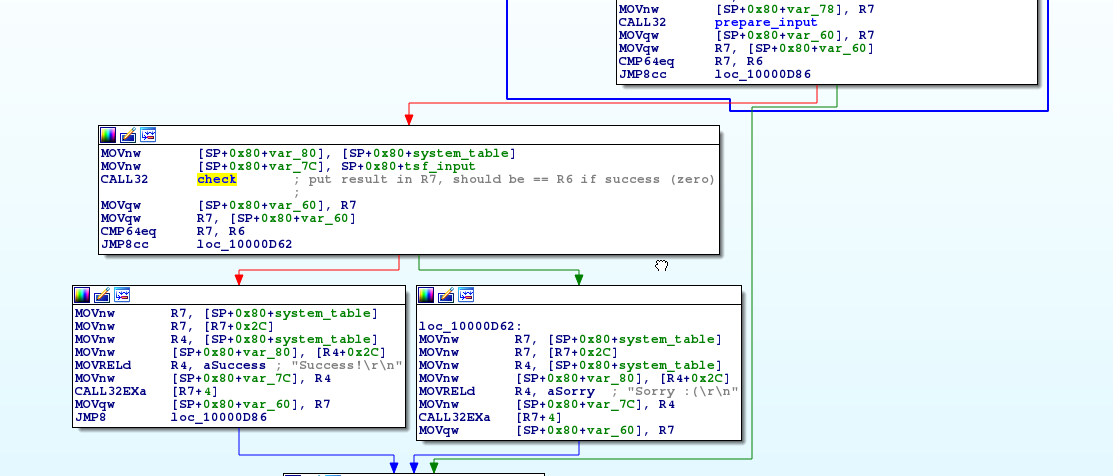
\includegraphics[width=0.8\textwidth]{./challs/part2/efi/img_check.png}
\centering
\end{figure}

La fonction {\em prepare\_input} vérifie la validité de l'input (on y trouve toutes les références aux chaînes du type "Invalid character...", "Key mus be exactly...").

{\em check} est plus intéressante. Le retour de la fonction est stocké dans le registre R7.
On va voir directement à la fin de la fonction pour voir comment est calculé R7.

\begin{figure}[H]
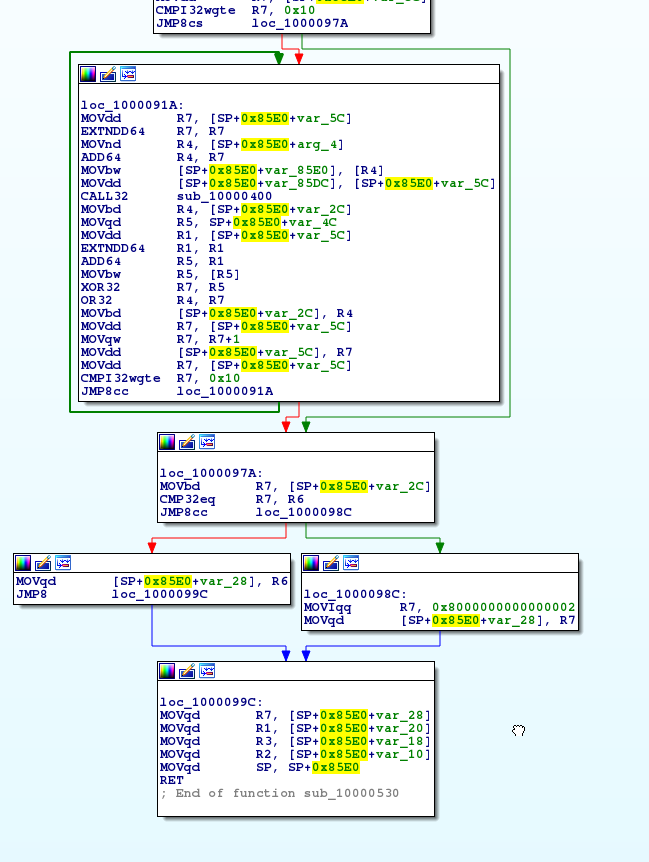
\includegraphics[width=0.8\textwidth]{./challs/part2/efi/img_loop.png}
\centering
\end{figure}

Jackpot, tout ce dont on a besoin se trouve dans ce snippet.
On a quelque chose du genre:
\begin{minted}{python}
for i in range(0x10):
  var_2c = var_2c | (input[i]^checkval[i])
R7 = 2 if var_2c else 0
# 0 for success
\end{minted}
Pas de timing attack donc (bien que je n'aurais pas su comment compter les instructions).

Deux options se présentent.
\begin{itemize}
\item \sout{ Reverser le décodage de {\em checkval}.}
\item On est une grosse feignasse et on automatise la résolution en patchant le compteur de la boucle pour trouver le résultat caractère par caractère.
\end{itemize}

La cible est l'instruction {.text:10000974 \em CMPI32wgte R7, 0x10}.
L'octet représentant le 0x10 se situe à 0x10000976.
Pour trouver l'offset dans le fichier, on exécute dans IDA python:
\begin{minted}{python}
idaapi.get_fileregion_offset(0x10000976)
# 2422
\end{minted}

On s'attend à devoir effectuer $2^{(7+4)}$ invocations du programmes pour trouver la bonne réponse.
Comme QEMU met des plombes à se lancer (j'ai pas réussi à désactiver PXE), c'est hors de question de le relancer à chaque fois.

Toutefois il est possible de faire passer les IO de QEMU à travers un pty.
On peut donc espérer construire quelque chose du style:
\begin{minted}{python}

ans_string=b'X'*0x10
for i in range(0x10):
  patch_file_with_end_condition(i+1)
  pty=launch_qemu()

  for j in range(0x256):
    ans_string[i]=j
    if pty.launch_program(ans_string).output.find("Success")!=-1:
      break
  else:
    assert 0
print(binascii.hexlify(ans_string))
\end{minted}

La solution en pratique est un peu différente. Comme l'EFI supporte les scripts, je génère un scipt qui effectue 256 appels à l'application avec chacun des candidates pour le caractère qu'on essaie de découvrir.

La solution complète peut être trouvée dans la section ressources.

La clé de challenge est {\em 347d8c72720d6ec7a501583be0bccc0c}

\subsubsection{Ressources}
\begin{itemize}
\item \textattachfile[mimetype=text/plain,color=0 0 0.5]{./challs/part2/efi/gen.py}{gen.py}
\end{itemize}



\FloatBarrier
\subsection{Huge}
\subsubsection{Sparse representation}
Extraction ELF avec la librairie do GO archive/tar/reader.go.
Unicorn engine pour faire tourner le binaire avec hooks et logs pour trouver les early exit rapidement.
\sout{Il se faisait tard et j'arrivais plus}... C'est vrai. cosinus bruteforce

\subsubsection{TL;WTL}
\begin{minted}{bash}
$ tar xvf huge.tar
Huge
tar: Huge: Cannot seek to 25297854992384: Invalid argument
tar: Exiting with failure status due to previous errors
$ # wut, j'ai jamais vu cette erreur. Listons le contenu de l'archive
$ tar -tvf huge.tar
-rwxr-xr-x 0/0 128574140715008 1970-01-01 01:00 Huge
$ # besoin d'un nombre pair de \$ pour vim :)
\end{minted}
%$
Ouf, on peut facilement imaginer des scénarios plus catastrophiques. Légère digression, je tournais pas sous VM pour les 2 premiers niveaux (si j'avais pu pour le 3ème, j'aurais continué :) ). Merci aux organisateurs de pas avoir (censément) mis de la merde dans les binaires.

Bon, même si le dés-archivage marche pas, tar nous sort gentiment le début du fichier.

\begin{minted}[breaklines]{bash}
$ file Huge
Huge: ELF 64-bit LSB exécutable, x86-64, version 1 (SYSV), statically linked, corrupted section header size
$ readelf --segments Huge
Elf file type is EXEC (Executable file)
Entry point 0x51466a42e705
There are 3 program headers, starting at offset 64

Program Headers:
  Type           Offset             VirtAddr           PhysAddr
                 FileSiz            MemSiz              Flags  Align
  LOAD           0x0000000000001000 0x00002b0000000000 0x00002b0000000000
                 0x00001ef000000000 0x00001ef000000000  R E    1000
  LOAD           0x00002afffffe1000 0x000049f000000000 0x000049f000000000
                 0x0000161000000000 0x0000161000000000  R E    1000
  LOAD           0x000049effffe1000 0x0000000000020000 0x0000000000020000
                 0x00002afffffe0000 0x00002afffffe0000  R E    1000
\end{minted}
Pas de WX, ouf! Par contre, ce sera pas du gâteau non plus.

\FloatBarrier
\paragraph{Récupérer les données}
Dans un premier temps il faut récupérer les différents bouts du fichier. En errant sur le web, on trouve que tar peut représenter des fichiers sparses. Encore une fois, j'ai pas envie de mettre le nez dans une quelconque spec. Patcher GNU tar, ce sera pour un autre jour. Ok, navigateur web, recherchons {\em tar sparse reader}. Tada, \url{https://golang.org/src/archive/tar/reader.go}.
Bien sûr les fonctions intéressantes ne sont pas exportées (shout out aux lowercases).
Tant pis, je copie le dossier complet de archive/* dans mon répertoire.
\inputminted{go}{./challs/part2/huge/archive/tar/test.go}

En pièce jointe: \textattachfile[mimetype=text/plain,color=0 0 0.5]{./challs/part2/huge/archive/tar/test.go}{archive/tar/test.go}

Le script me pond un fichier json avec chaque entrée de la sparse table.

\FloatBarrier
\paragraph{Trouver la clé}
Ok, on a le contenu de l'elf mais aucun moyen de l'exécuter. Rebelotte, j'ai pas envie de reverser le fichier.
L'espace d'adressage virtuel de l'elf est contigu avec le contenu mémoire à zéro hormis pour les morceaux qu'on a extrait de la sparse table.
On va donc se manger pleins d'instructions type \mintinline{asm}{add byte ptr [rax], al} ('\textbackslash x00\textbackslash x00').
Ya des chances qu'on puisse ignorer ces opérations (ou du moins les compresser (genre si on a N instructions de ce type, on a juste à exécuter $N \mod 256$ instructions puis sauter à la prochaine instruction intéressante.)

Une solution possible est de patcher le header elf pour modifier les champs Offset et FileSiz en mettant les entrées sparse bout à bout. En scriptant gdb il serait possible de hook les segfaults et effectuer les jump nous même.

Mais non.

\textbf{<histoire fantastique>} Il y a de cela quelques mois, je me suis attaqué à la résolution d'un crackme. Ce crackme fort obfusqué, exécutaient ses instructions à travers sa propre VM (outre plus,  les points d'arrêts n'étaient pas facilité de par la vérification de l'intégrité du code (d'abondant, mes breakpoints matériels me donnaient de joli SIGBUS, pour raison que j'ignore encore)). De par ma flemme de reverser se binaire, \textbf{</histoire fantastique>} j'avais été amené à utiliser \url{http://www.unicorn-engine.org/}.
En gros c'est un émulateur multi-architectures basé sur QEMU où on peut foutre autant de hooks (mémoire, code, interrupt) qu'on veut.

En plus comme l'elf qu'on a ne fait que des syscalls triviaux (read, write et exit), on a quasiment rien à émuler nous même. Le seul taff à faire est de charger l'elf, mettre les hooks entre les entrées sparse et avoir un système de log décent pour naviguer facilement la trace.

Fâcheusement c'est pas une solution automatique mais comme le binaire est en early exit on s'en sort. En rétrospective il aura d'ailleurs été possible d'employer une timing attack puisque les vérifications se font par groupe de 4 octets au maximum, mais comme le système de trace était assez joli, l'identification des conditions fut très rapide.

Voici une explication du déroulement du programme:

Bonne nouvelle, unicorn fonctionne bien :)
\begin{minted}[breaklines]{text}
CODE at  0x51466a42e731 b'0f05'
0x51466a42e731:	syscall	 bytearray(b'\x0f\x05')
[1, 99265643088311, 27] #rdi, rsi, rdx
GOT HOOK >>  write
WRITING >>  bytearray(b'Please enter the password: ')

...


CODE at  0x51466a42e741 b'0f05'
0x51466a42e741:	syscall	 bytearray(b'\x0f\x05')
[0, 1108992, 1024]
GOT HOOK >>  read
# note: ici on écrit ce qu'on veut

... Lecture de notre buffer

0x10f338cf754d: movzx ebx, byte ptr [rsi]      <<<< TRACEVENT, rax=0010ec00
OpReg ebx:00000000 
ReadEvent addr:000000000010ec00 n:0000000000000001 val:0000000000000032 
Regs
rbx:0000000000000000 
rbx:0000000000000032 

0x10f338cf7550: sub bl, 0x30     <<<< TRACEVENT, rax=0010ec00
OpReg bl:32 
Regs
rbx:0000000000000032 
rbx:0000000000000002 

... On réécrit dans le même buffer le unhexlify

0x10f338cf75a4: mov byte ptr [rdi], bl 		 <<<< TRACEVENT, rax=0010ec00
OpReg bl:29 
WriteEvent addr:000000000010ec00 n:0000000000000001 nval:0000000000000029 val:0000000000000032 
Regs
\end{minted}

Avec ses quelques logs, on voit que l'on s'attend à ce que nos données soient une chaine hexa et qu'on le \mintinline{python}{binary.unhexlify} stocke le résultat dans le même buffer.


\begin{minted}[breaklines]{text}
-- First check :
0x43abdb4a0af9: cmp byte ptr [rsp], 0x29 		 <<<< TRACEVENT, rax=0010ec00
ReadEvent addr:000000000010ec00 n:0000000000000001 val:00000000000000aa 
-> 29XXXXXX

======================

-- Second check :
0x4a170682ede1: cmp word ptr [rsp + 2], 0xd17e 		 <<<< TRACEVENT, rax=0010ec00
ReadEvent addr:000000000010ec02 n:0000000000000002 val:000000000000aaaa 
-> 29XX7ED1

======================

-- Third check :
0x6f4b0e0f370: cmp byte ptr [rsp + 0xb], 0x8c 		 <<<< TRACEVENT, rax=0010ec00
ReadEvent addr:000000000010ec0b n:0000000000000001 val:00000000000000aa 
-> buf[0xb] = 0x8c

======================

-- Fourth check: 
0x49e7e541be22: movzx rbx, byte ptr [rsp + 9]      <<<< TRACEVENT, rax=0010ed03
OpReg rbx:000049e7e541000c 
ReadEvent addr:000000000010ec01 n:0000000000000001 val:00000000000000aa 
rbx:000049e7e541000c 
rbx:00000000000000aa 

0x49e7e541be28: mov byte ptr [rax], 0 		 <<<< TRACEVENT, rax=0010ed03
WriteEvent addr:000000000010ed03 n:0000000000000001 nval:0000000000000000 val:0000000000000000 

0x49e7e541be2b: lea rcx, qword ptr [rip + 6] 		 <<<< TRACEVENT, rax=0010ed03
OpReg rcx:0000000000000000 
rcx:0000000000000000 
rcx:000049e7e541be38 

0x49e7e541be32: lea rcx, qword ptr [rcx + rbx*2] 		 <<<< TRACEVENT, rax=0010ed03
OpReg rcx:000049e7e541be38 
rcx:000049e7e541be38 
rcx:000049e7e541bf8c 

0x49e7e541be36: jmp rcx 		 <<<< TRACEVENT, rax=0010ed03
OpReg rcx:000049e7e541bf8c 

0x49e7e541bf8c: add byte ptr [rax], al 		 <<<< TRACEVENT, rax=0010ed03
OpReg al:10ed03 
ReadEvent addr:000000000010ed03 n:0000000000000001 val:0000000000000000 
WriteEvent addr:000000000010ed03 n:0000000000000001 nval:0000000000000003 val:0000000000000000 
+++++++++++++++++ Multiple iterations here

0x49e7e541c038: cmp byte ptr [rax], 0x65 		 <<<< TRACEVENT, rax=0010ed03
ReadEvent addr:000000000010ed03 n:0000000000000001 val:0000000000000002 
Regs
-> buf[1] = 0x89
\end{minted}

Voici le raisonnement pour que la quatrième condition soit vérifiée:
\begin{itemize}
\item byte ptr[rax]=0
\item al = 3 -> on ajout 3 a chaque add byte ptr [rax], al
\item On veut a la fin que byte ptr [rax] = 0x65. 
\item On doit exécuter $65_{16} / 3 \equiv 119 \mod 256$
\item Sur les 256 instructions exécutées au maximum, on en saut buf[1].
\item On veut donc $buf[1] = 256 - 119 = 89_{16}$.
\end{itemize}

\begin{minted}[breaklines]{text}
-- Fifth check:
0x352845ab3bd5: xor ebx, dword ptr [rsp + 0xc] 		 <<<< TRACEVENT, rax=0010ec00
OpReg ebx:352845ab3bd5 
ReadEvent addr:000000000010ec0c n:0000000000000004 val:00000000aaaaaaaa 
Regs
rbx:0000352845ab3bd5 
rbx:00000000ef01917f 

0x352845ab3bd9: cmp ebx, 0xa9b00f5c 		 <<<< TRACEVENT, rax=0010ec00
OpReg ebx:ef01917f 
Regs
-> buf[0xc -> 0x10] = 0xec1b3489 = 0xa9b00f5c ^ 0x45ab3bd5

=======

-- Sixth check:
0x59cb440c4536: mov eax, dword ptr [rsp + 0x10] 		 <<<< TRACEVENT, rax=8caaaaaa
OpReg eax:0010ec00 
ReadEvent addr:000000000010ec08 n:0000000000000004 val:000000008caaaaaa 
Regs
rax:000000000010ec00 
rax:000000008caaaaaa 


0x59cb440c453a: xor rax, rbx 		 <<<< TRACEVENT, rax=59cb4466a129
OpReg rax:000000008caaaaaa rbx:000059cbc8cc0b83 
Regs
rax:000000008caaaaaa 
rax:000059cb4466a129 


0x59cb440c453d: movabs rbx, 0x2a7ee24a000c 		 <<<< TRACEVENT, rax=59cb4466a129
OpReg rbx:000059cbc8cc0b83 
Regs
rbx:000059cbc8cc0b83 
rbx:00002a7ee24a000c 


0x59cb440c4547: cmpxchg rcx, rbx 		 <<<< TRACEVENT, rax=59cb440c4556
OpReg rbx:00002a7ee24a000c rcx:000059cb440c4556 
Regs
rax:000059cb4466a129 
rax:000059cb440c4556 
Want rax = rax -> buf[0x8] = 0xc8cc0b83 ^ 0x440c4556  = 0x8cc04ed5
\end{minted}


Pour la dernière vérification des instructions pour nombres à virgule sont utilisées. 

\begin{minted}[breaklines]{text}
0x2a7ee24aae3d: xor dword ptr [rsp + 0x1c], ebx 		 <<<< TRACEVENT, rax=0010ec00
OpReg ebx:aaaaaaaa 
ReadEvent addr:000000000010ec14 n:0000000000000004 val:0000000024b87838 
WriteEvent addr:000000000010ec14 n:0000000000000004 nval:000000008e12d292 val:0000000024b87838 
Regs

0x2a7ee24aae41: wait  		 <<<< TRACEVENT, rax=0010ec00
Regs

0x2a7ee24aae42: fnclex  		 <<<< TRACEVENT, rax=0010ec00
Regs

Content of [rsp+0x18] b'cb6d711eecae34bdfe3f333431626563'
0x2a7ee24aae44: fld xword ptr [rsp + 0x18] 		 <<<< TRACEVENT, rax=0010ec00
Regs

CODE at  0x2a7ee24aae44 b'db6c2418'
0x2a7ee24aae44:	fld	xword ptr [rsp + 0x18] 

0x2a7ee24aae48: fld st(0) 		 <<<< TRACEVENT, rax=0010ec00
Regs

0x2a7ee24aae4a: fcos  		 <<<< TRACEVENT, rax=0010ec00
Regs

0x2a7ee24aae4c: fcompp  		 <<<< TRACEVENT, rax=0010ec00
Regs

0x2a7ee24aae4e: wait  		 <<<< TRACEVENT, rax=0010ec00
Regs

0x2a7ee24aae4f: fnstsw ax 		 <<<< TRACEVENT, rax=00100000
OpReg ax:10ec00 
Regs
rax:000000000010ec00 
rax:0000000000100000 
\end{minted}

On vérifie que $x=quad\_float(rsp + 0x18) : x=cos(x) -> x\approx 0.739085$.


Rien de mieux qu'un
\begin{minted}[breaklines]{cpp}
int main() {
  for (u64 i = 0; i < 1ull << 32; ++i) {
    u64 a = 0x1e716dcb + (i << 32);
    u64 b = 0x6365623134333ffe;
    u64 res;

    // ok at 3174346476
//a=0xbd34aeec1e716dcbull;
//b=0x6365623134333ffeull;
    __asm__ volatile("mov rax, %2\n"
                     "pushq rax\n"
                     "mov rax, %1\n"
                     "pushq rax\n"
                     "wait\n"
                     "fnclex\n"
                     "fld tbyte ptr [rsp]\n"
                     "fld st(0)\n"
                     "fcos\n"
                     "fcompp\n"
                     "wait\n"
                     "fnstsw ax\n"
                     "and rax, 0xffdf\n"
                     "mov %0, rax\n"
                     "popq rax\n"
                     "popq rax\n"
                     : "=r"(res)
                     : "r"(a), "r"(b)
                     : "%rax");

    if (res == 0x4000) {
      printf("ok at %Lu\n", i);
    }
  }
  return 0;
}
\end{minted}
La programme trouve la solution pour $i=3174346476 \implies buf[0x4:0x8]=3174346476 \oplus 0x24b87838=0x998cd6d4$
L'input que l'on doit spécifier est {\em 29897ed1d4d68c99d54ec08c89341bec}.

Petit bémol, QEMU se rate sur le fcompp et me retourne fail. J'ai pas creusé pourquoi, mais en ignorant le fail jump, j'obtiens:

\begin{minted}[breaklines]{text}
CODE at  0x99a380575e2 b'0f05'
0x99a380575e2:	syscall	 bytearray(b'\x0f\x05')
[1, 99265643088338, 12]
GOT HOOK >>  write
WRITING >>  bytearray(b'The key is: ')

 ---

CODE at  0x99a380575f3 b'0f05'
0x99a380575f3:	syscall	 bytearray(b'\x0f\x05')
[1, 1108992, 32]
GOT HOOK >>  write
WRITING >>       bytearray(b'E574B514667F6AB2D83047BB871A54F5')
\end{minted}

La clé de ce niveau est {\em E574B514667F6AB2D83047BB871A54F5}

\subsubsection{Ressources}
\begin{itemize}
\item \textattachfile[mimetype=text/plain,color=0 0 0.5]{./challs/part2/huge/archive/tar/test.go}{test.go}
\item \textattachfile[mimetype=text/plain,color=0 0 0.5]{./challs/part2/huge/solve.py}{Solver} -> des librairies perso sont utilisées mais ça peut quand même donner une idée.
\item \textattachfile[mimetype=text/plain,color=0 0 0.5]{./challs/part2/huge/traces/events.out}{Trace events}
\item \textattachfile[mimetype=text/plain,color=0 0 0.5]{./challs/part2/huge/traces/res.out}{Trace output}
\item \textattachfile[mimetype=text/plain,color=0 0 0.5]{./challs/part2/huge/find.cpp}{cosinus finder}
\inputminted{go}{./challs/part2/huge/archive/tar/test.go}
\end{itemize}


\section{Niveau 3, Floating through long wasted days}

Quatre challenges ce coup-ci, Une brève discussion des
\begin{itemize}
\item[video] Récupérer des données exfiltrés par un fond d'écran dont on a les sources.
\item[usb] Appli avec windows driver qui cache des données entre des partitions d'un disque. Trouver qu'elles sont ces données à partir d'une image et de l'encodeur.
\item[ring 2x] Application win64 fait tourner sa propre vm. Décodage des instructions se fait par des child process qui pilotent le parent à travers le débuggeur (chaine de 8 process il me semble). Pas de possibilité de s'attacher, sauf avec un débuggeur noyau. Y'a aussi l'air d'avoir des vérifications de timing (perf counters), donc c'est pas sur que ca marche non plus.
\item[strang 2x] Itanium elf. Voila.
\end{itemize}

ring à l'air super intéressant, je l'aurais bien essayé si seulement win64 fonctionnait sans kvm dans qemu.

\subsection{video}
\subsubsection{Regarder la vidéo}
Non vraiment, le reste c'est du travail manuel.

\subsubsection{Un jour j'irais droit au but}

Première chose à faire, c'est d'essayer de lancer le programme. Après ca on pourra attacher un débuggeur pour reverser plus rapidement. Bien sûr c'est pas si facile: d'abord des problèmes de résolution et ensuite juste rien qui s'affiche à l'écran.
J'ai bien envie de voir les images même si c'est pas du tout nécessaire pour résoudre le challenge.

Rien de mieux que de créer ma propre {\em ddraw.dll} et d'écrire les images dans un fichier. Ca ressemble à ca:

\begin{minted}{cpp}
MyDirectDraw g_draw;

HRESULT WINAPI DirectDrawCreate(
    _In_  GUID FAR         *lpGUID,
    _Out_ LPDIRECTDRAW FAR *lplpDD,
    _In_  IUnknown FAR     *pUnkOuter
    ){
  log_file << "KAPPA";
  log_file.flush();
  *lplpDD = &g_draw;
  int *is_activate = (int*)0x0040F0E0;
  *is_activate = 1;


  return 0;
}
\end{minted}


\begin{listing}[H]
  \caption{lib.def}
  \inputminted{text}{./challs/part3/video/Stage_anti_APT_chez_Airlhes/win/lib/lib.def}
\end{listing}

En gros j'ai juste besoin d'exporter la fonction {\em DirectDrawCreate} et de fournir une interface {\em IDirectDraw} potable.

Magnifique résultat:
\begin{figure}[H]
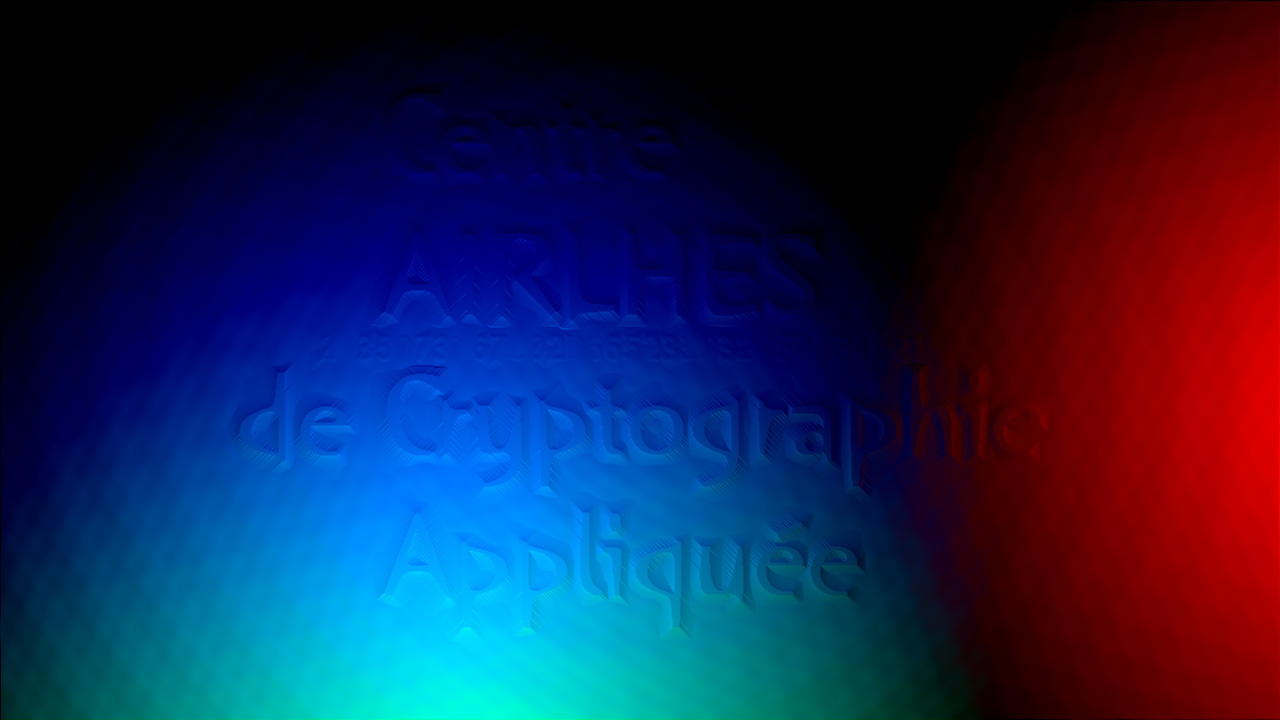
\includegraphics[width=0.8\textwidth]{./challs/part3/video/Stage_anti_APT_chez_Airlhes/win/res_0012.png}
\centering
  \label{video:img_screen}
\end{figure}

En vidéo ca fait 3 spotlights RGB qui se déplacent lentement. Très bien ca explique le début de la vidéo mais pas les brusques changement de couleurs. Il est l'heure de reverser tout ca plus proprement.

  \par Dans les fonctions importées, on observe {\em RegEnumValueA, RegOpenKeyExA} mais pas de primitives de lecture de fichier. C'est probablement une clé de registre qui va être exfiltrée. En regardant les Xref, on tombe sur:

\begin{figure}[H]
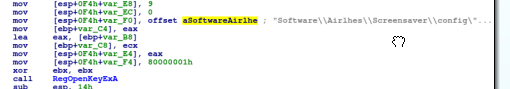
\includegraphics[width=0.8\textwidth]{./imgs/video_reg1.png}
\centering
\end{figure}

En mettant des points d'arrêts mémoire, on arrive à trouver où est utilisé le buffer de lecture du registre: .text:00403500, une fonction lancée dans un thread.
Voici le traitement réalisé sur un octet du registre.
\begin{minted}[breaklines]{python}

color_tb=something # static data, taille 8
cur_idx=something_else # pour premier char, 6
  reg_char=read() ^ xorpad[cur_step] # xorpad en static data
for i in range(3):
  cur_idx += reg_char % 7 + 1
  reg_char = reg_char // 7 + 1
  push(color_tb[cur_idx]) # envoyer données au thread principal
\end{minted}

  Cette partie explique bien ce qu'on voit dans la vidéo: des flashs de couleur successifs, avec la même durée. On a pas de répétition d'un même couleur grâce à l'accumulateur cur\_idx et au mod 7 {\em + 1}.
Bien évidemment, j'ai passé trop de temps sur le mod 7. Pour cela, je tiens à exprimer ma gratitude à l'opération div pour toujours se faire dégager par les optimisations compilo.


On poursuit notre route dans le thread principal, là où les données sont récupérées.

\begin{figure}[H]
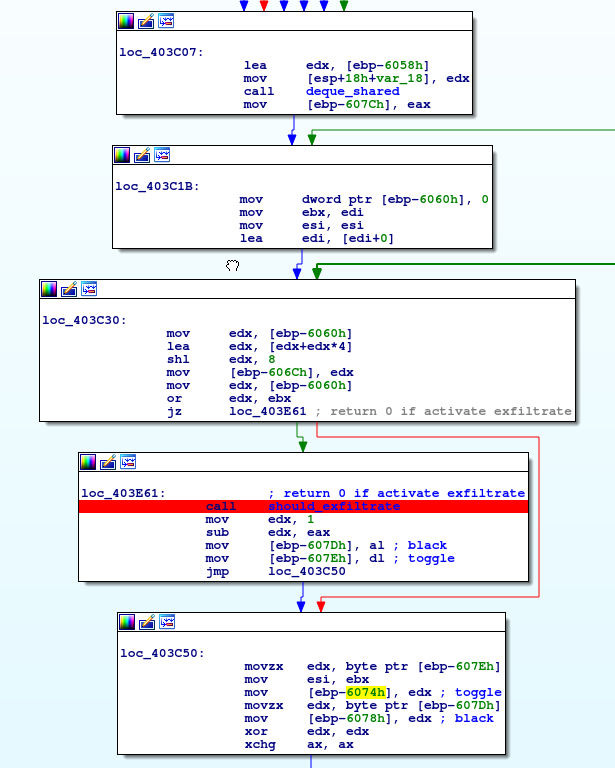
\includegraphics[width=0.8\textwidth]{./imgs/video_final_logic.png}
\centering
\end{figure}

\begin{figure}[H]
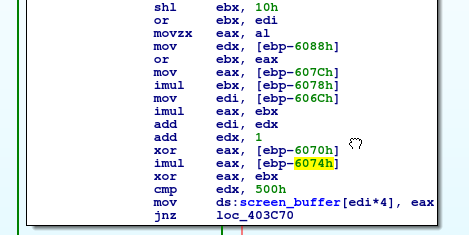
\includegraphics[width=0.8\textwidth]{./imgs/video_final_logic2.png}
\centering
\end{figure}

\paragraph{Brève parenthèse autour de la fonction should\_exfiltrate}
  Avec le débuggeur, cette fonction m'a toujours retourné 1. En ouvrant la fonction, on voit des appels à GetLocaltime et SystemTimeToFileTime. En se replacant dans le contexte générale, notre cible est un écran de veille qui exfiltre des données en changeant rapidement de couleurs. Dans la vidéo on peut voir deux modes d'opérations, le mode standard (\ref{video:img_screen}) et un mode de succession rapdie de couleurs. Avec ces appels de fonctions, on se doute que le second mode se déclenche dans une certaine plage horaire. Bien sur, le code de la fonction est plein de opérations sur flottants. Non merci. Pour trouver la plage horaire, la flemme de modifier l'heure système. Ya peu de candidat, mais j'ai une flemme monstre. Un petit script ida python et c'est parti

\begin{minted}[breaklines]{python}
class Hooker(idaapi.DBG_Hooks):
  def __init__(self, data):
    super(Hooker, self).__init__()
    self.done = False
    self.exited = False
    self.data = data

    self.test_time_func = idc.LocByName('should_exfiltrate')
    self.test_time_start = idc.LocByName('loc_403E61')
    self.test_time_end=0x00403E66
    self.test_time_mod=0x00403767
  def dbg_bpt(self, tid, ea):
    elif ea==self.test_time_end:
      if self.time>=3600*24:
        self.done=1
        #entre 23h et 1h
      else:
        idautils.cpu.eip=self.test_time_start
        resv=idautils.cpu.eax
        h,m,s=self.get_time(self.time)
        print 'REsult: %d:%d:%d >> %d'%(h,m,s,resv)
        self.time+=60

    elif ea==self.test_time_mod:
      h,m,s=self.get_time(self.time)
      addr=idautils.cpu.ebx
      write_u16(addr+4*2, h)
      write_u16(addr+5*2, m)
      write_u16(addr+6*2, s)

  def get_time(self, t):
    return t/3600, t/60%60, t%60
\end{minted}

Résultat, le exfiltration se déclenche entre 23h et 1h.


\paragraph{De retour à nos moutons}
La fonction {\em should\_exfiltrate} retourne 0 pour le mode caché.
En suivant les variables, on va donc avoir dans ce mode:
\begin{minted}[breaklines]{text}
edx = 1
[ebp-607d] = 0
[ebp-607E] = 1
[ebp-6074] = 1
[ebp-6078] = 0
...
col_id_from_other_thread aka A = [ebp-607c]
ebx = 0 = ebx * [ebp-6078] // WUT, why not used??
eax = 0 = eax *e bx
eax ^= [ebp - 6070]
eax = old_eax = eax * [ebp-6074]
screen_buffer[_] = old_eax = eax ^ ebx
\end{minted}
Ok, bizarre notre caractère est ignoré.
Par contre on a un autre candidate prometteur en [ebp-6070].

\begin{figure}[H]
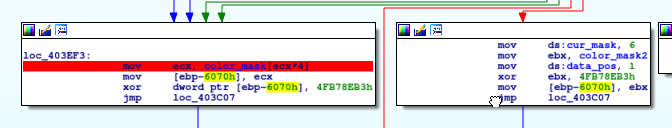
\includegraphics[width=0.8\textwidth]{./imgs/video_trap.png}
\centering
\end{figure}

En regardant dans cette zone, on voit un code bien similaire à celui du thread qui nous envoie les données. J'aurais peut-être pas du m'arrêter au premier hardware breakpoint pour le buffer du registre.
Le code possède une logique éguivalente.

\begin{minted}[breaklines]{python}

color_tb=something # static data, taille 8
cur_idx=something_else # pour premier char, 6
  reg_char=read() ^ xorpad[cur_step] # xorpad en static data
for i in range(3):
  cur_idx += reg_char % 7 + 1
  reg_char = reg_char // 7
  push color_tb[cur_idx]
\end{minted}

Bon, on sait maintenant comment le tout fonctionne. Un préambule avec écran BLANC NOIR BLANC et ensuite le défilement de couleurs correspondant aux données à exfiltrer.
On regarde la vidéo en notant les chacune des 8 couleurs possibles (j'ai pas sorti opencv :) ).
Ensuite on trouve les données envoyés caractère par caractère en vérifiant avec les couleurs observés.
Un code python ignoble pour résoudre le tout est dispo en ressources.

\begin{minted}{bash}
$ python analyse.py
...
b'1800000078da0b1634172bdac558f9cb6e6257f3be7b5b003250077e'
$ file /tmp/res.out
/tmp/res.out: zlib compressed data
$ printf "\x1f\x8b\x08\x00\x00\x00\x00\x00"  | cat - /tmp/res.out | zcat - | xxd
gzip: stdin: unexpected end of file
00000000: 5311 3716 72ba 0179 fa3e 918a 83be deb4  S.7.r..y.>......
$ #
\end{minted}

\begin{minted}{text}
Clé: 5311371672ba0179fa3e918a83bedeb4
\end{minted}

\subsubsection{Ressources}

\begin{itemize}
\item \textattachfile[mimetype=text/plain,color=0 0 0.5]{./challs/part3/video/Stage_anti_APT_chez_Airlhes/analyse.py}{analyse.py}
\item \textattachfile[mimetype=text/plain,color=0 0 0.5]{./challs/part3/video/Stage_anti_APT_chez_Airlhes/win/lib/lib.cpp}{lib.cpp}
\item \textattachfile[mimetype=text/plain,color=0 0 0.5]{./challs/part3/video/Stage_anti_APT_chez_Airlhes/win/lib/lib.h}{lib.h}
\item \textattachfile[mimetype=text/plain,color=0 0 0.5]{./challs/part3/video/Stage_anti_APT_chez_Airlhes/win/lib/lib.def}{lib.def}
\item \textattachfile[mimetype=text/plain,color=0 0 0.5]{./challs/part3/video/Stage_anti_APT_chez_Airlhes/win/lib/ddraw.h}{ddraw.h}
\item \textattachfile[mimetype=text/plain,color=0 0 0.5]{./challs/part3/video/Stage_anti_APT_chez_Airlhes/win/CMakeLists.txt}{CMakeLists}
\item \textattachfile[mimetype=text/plain,color=0 0 0.5]{./challs/part3/video/Stage_anti_APT_chez_Airlhes/Airlhes_screensaver.idb}{IDA db}
\item + lodepng trouvable sur le net
\end{itemize}


\subsection{usb}
\subsubsection{Biographie}
Reverse du code. Seul le driver est intéressant.
Données dans les parties non allouées du disque.
RC4 par fichier + RC5 sur tout le flux.

Les fichiers IDA avec commentaire sont disponibles dans la section ressources \ref{usb_resources}.
\subsubsection{Autobiographie}

On nous donne deux fichiers, un binaire windows et une image disque.

\begin{minted}[breaklines]{bash}
$ file img
img: DOS/MBR boot sector; partition 1 : ID=0xb, start-CHS (0x0,0,4), end-CHS (0x88,233,5), startsector 3, 2097152 sectors; partition 2 : ID=0xb, start-CHS (0x89,19,6), end-CHS (0xcd,135,36), startsector 2099201, 1048575 sectors; partition 3 : ID=0xb, start-CHS (0xcd,135,38), end-CHS (0xce,218,57), startsector 3147777, 20480 sectors; partition 4 : ID=0xb, start-CHS (0xce,218,58), end-CHS (0x14,93,50), startsector 3168257, 819199 sectors
$ #
\end{minted}

En montant les différentes partitions, on trouve aucun fichier intéressant (un pdf, mais peu de chance que y'ait des données cachées dedans.) Il est plus probable que les données soient stockées ailleurs.
On peut ouvrir le fichier avec \href{Autopsy}{http://www.sleuthkit.org/autopsy/}.

\begin{figure}[H]
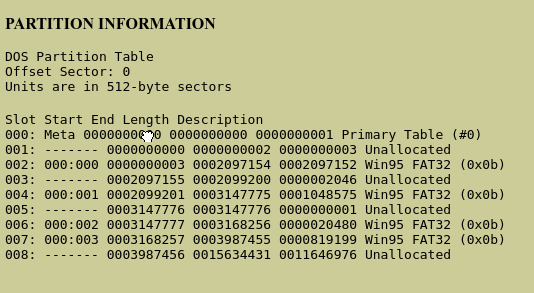
\includegraphics[width=0.8\textwidth]{./imgs/usb_img_partitions.png}
\centering
\end{figure}
Plusieurs secteurs non alloués. Ca peut-être intéressant. Les 3 premiers secteurs:
\begin{figure}[H]
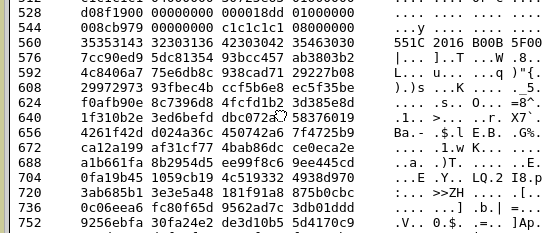
\includegraphics[width=0.8\textwidth]{./imgs/usb_img_data1.png}
\centering
\end{figure}

Bingo une chaîne de caractère {\em 551C 2016 B00B 5F00}. Par contre les données ont l'air aléatoire, faut maintenant étudier le programme et on verra si on croise cette chaine plus tard.\\

Exécuter le programme ne fonctionne pas. En regardant ce qu'il se passe avec Process Monitor, on voit que le binaire essaie de lancer un service. En extrayant les ressources du PE, on obtient le fichier {\em userSSTIC\_101\_BINARY.bin}. Ce fichier est un module noyau windows et on suppose que c'est celui qu'on essaie de lancer avec les appels à {\em CreateService} et {\em StartService}.

\paragraph{Le binaire userspace \\ }

Les fonctions importées par le binaire nous permettent de trouver rapidement les fonctions intéressantes.
\begin{figure}[H]
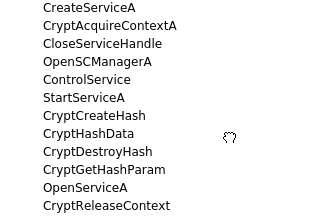
\includegraphics[width=0.8\textwidth]{./imgs/usb_binary_imports.png}
\centering
\end{figure}

En jetant un oeil aux endroits qui font appel aux fonction crypto, on déduit un algorithme du genre:
\begin{algorithm}[h]
  \For{ Tous les fichiers f dans "\textbackslash SSTIC\textbackslash * } {
    Attendre l'event 1 (signalant que le driver est prêt pour le prochain fichier)
    Lire F et calculer son MD5 et placer le tout dans un buffer à une adresse fixe (format [HASH|CONTENT])
    Signaler l'event 2, pour dire que le fichier est prêt.
  }
\end{algorithm}

En cherchant l'initialisation de l'adresse fixe, on voit qu'elle n'est pas initialisée dans l'application.
\begin{figure}[H]
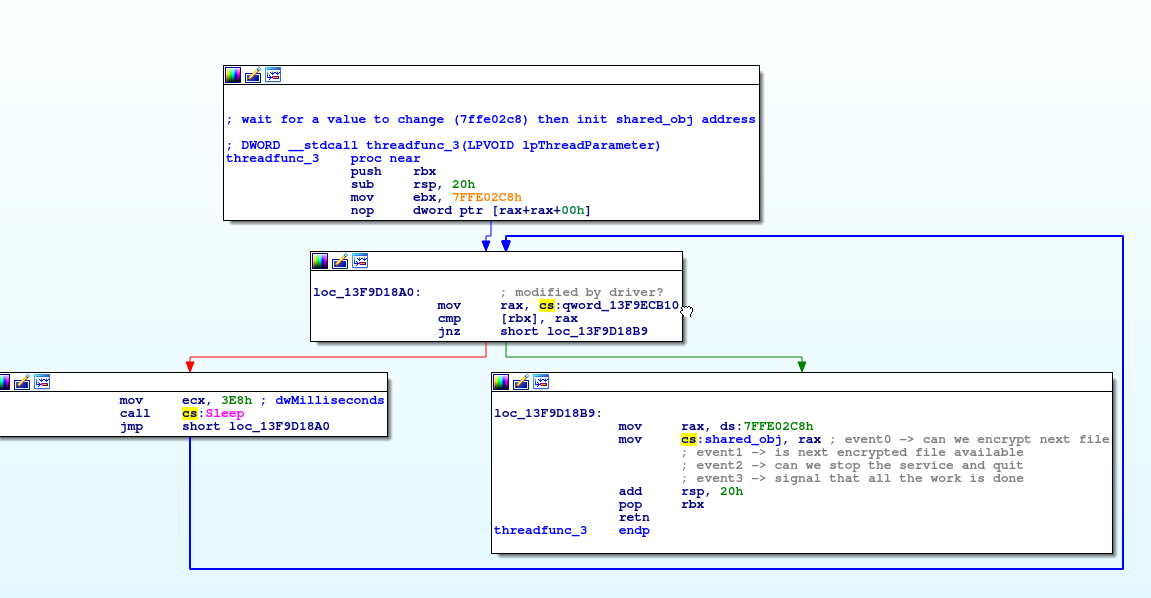
\includegraphics[width=0.8\textwidth]{./imgs/usb_binary_wait_driver_init.png}
\centering
\end{figure}

On observe aussi dans le binaire que les events ne sont utilisés que dans une direction.
Tout cela nous amène à penser que le c'est le driver qui s'occupera de faire quoi que ce soit avec ces fichiers + hash et que la communication se fait par mémoire partagée + events.


Une autre pièce du puzzle dans le binaire userspace réside dans la gestion des évènements win32.
\begin{figure}[H]
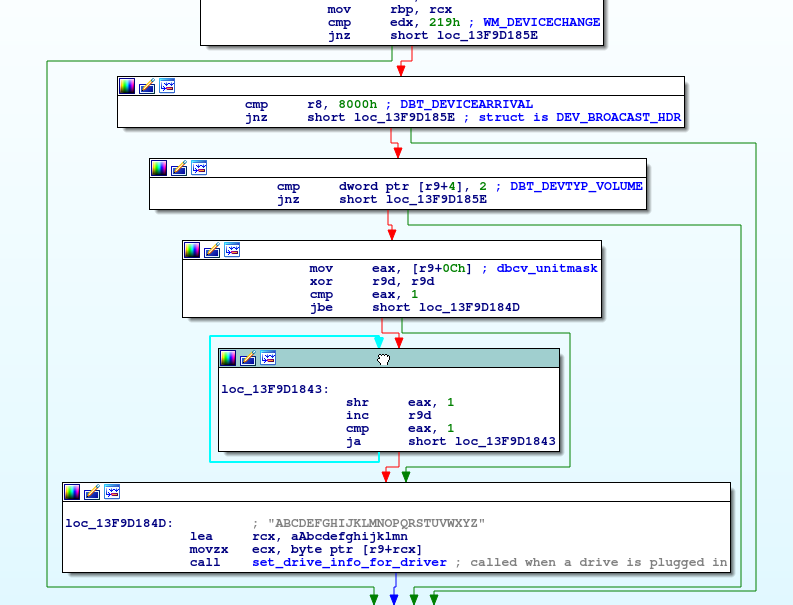
\includegraphics[width=0.8\textwidth]{./imgs/usb_binary_wait_new_disk.png}
\centering
\end{figure}
Une fois qu'un nouveau disque est détecté, on appel la fonction ici nommée set\_drive\_info\_for\_driver qui se charge de transmettre la lettre du disque qui vient d'être branché au driver.


Il n'y a plus grand chose d'intéressant dans le l'application. Il est temps d'aller jeter un oeil au driver.

\paragraph{Le driver\\ }

Comme on sait que l'application et le driver se synchronise à travers des events, il est utile de se diriger vers les fonctions importées type {\em KeWaitForSingleObject} ou {\em KeSetEvent}. Cela nous permet d'identifier directement la zone de mémoire partagée avec l'application (le pointer se trouve à {\em .data:0000000000215188}.)

On regarde ensuite les Xref de ce pointeur. On y identifie facilement les fonctions de synchronisations avec l'application, la fonction de création de la mémoire partagée (.text:0000000000011078) et la fonction la plus intéressant, là où le buffer du fichier est traité (.text:000000000001110C).

Dans cette fonction, on observe un PRNG seedé avec une variable 32 bit qui est utilisé pour générer 16 octets.
Une permutation générée à partir des octets précédents. À ce moment, je me dis qu'il faut que je reverse cet algo comme je vais devoir décoder l'image disque qu'on nous a fourni. Après avoir annoté tout l'algo qui génère la permutation, je clique: RC4. Ca m'évite de devoir réverser la génération du stream cipher.

Dans la suite de la fonction, le buffer encodé est copié dans un nouveau buffer avec de nouvelles informations sous le format:
\begin{minted}[breaklines]{text}
  [NEXT:8|PREV:8|BLK_SIZE:4|FILE_SIZE:4| RC4_KEY:0x10|MD5_HASH:0x10|RC4_ENC_BUF_PTR:0x10]
\end{minted}
La clé RC4 est conservée, youhou on aura pas à la bruteforce.
On identifie que ce buffer est foutu dans une liste chaîné avec la première entrée (ou sentinelle, j'ai pas regardé plus loin) situé en .data:0000000000015120.

La fonction se termine. Il faut maintenant s'intéresser aux endroits où est utilisée la liste chaînée.
Xref à nouveau, on tombe sur la fonction .text:0000000000013020.

La fonction commence par itéré sur les éléments de liste pour calculer la taille totale du buffer (champs à 0x10). Puis on alloue un buffer de cette taille. Ok, on va donc concaténer tous les [size|RC4\_KEY|ENC\_MD5|ENC\_BUF].

Un peu plus loin on voit en effet:
\begin{figure}[H]
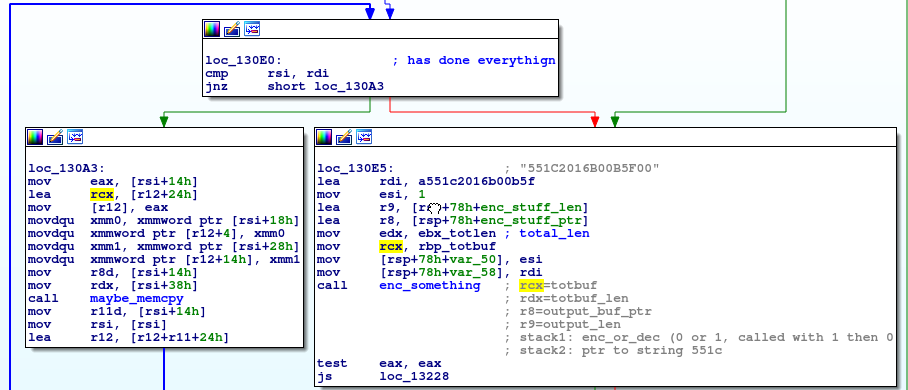
\includegraphics[width=0.8\textwidth]{./imgs/usb_driver_concat_rc5.png}
\centering
\end{figure}

La boucle concatène les chunks et on appelle une fonction sur le gros buffer (rbp\_totbuf).
Étudions cette fonction. Le première appel de fonction intéressant est en .text:00000000000121FE. On remarque que la chaîne de caractère "551C2016B00B5F00" est en argument et donc ca devrait forcément faire quelque chose d'intéressant.

Dans cette fonction, on découvre:
\begin{figure}[H]
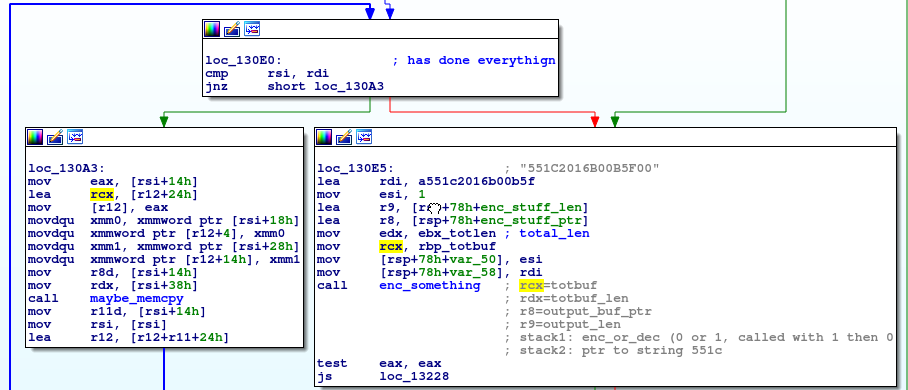
\includegraphics[width=0.8\textwidth]{./imgs/usb_driver_concat_rc5.png}
\centering
\end{figure}

De la crypto, cool. Une constante, encore plus cool. Moteur de recherche sur {\em B7E15163}, on tombe sur RC5.
Le programme fait donc tourner un RC5 sur le gros buffer.

On poursuit l'exécution du programme, et on tombe sur une très jolie fonction:
\begin{figure}[H]
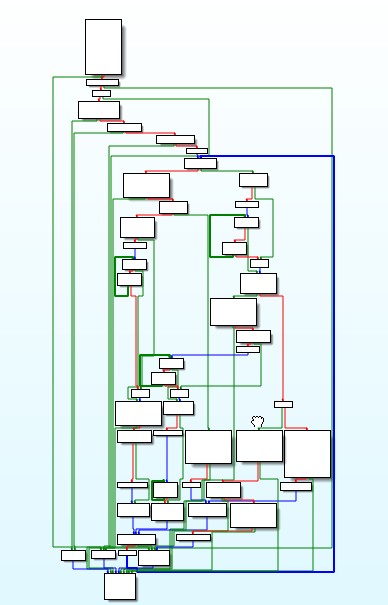
\includegraphics[width=0.8\textwidth]{./imgs/usb_driver_write_fat.png}
\centering
\end{figure}

Ok, pas moyen que je reverse ca. On va plutôt essayer de déduire ce que ca fait.
On sait déjà que notre programme va écrire nos données encryptées sur le disque.
Un fonction importée par le driver qui pourrait être capable de faire ca est {\em IofCallDriver}.
Cette fonction est notamment appelée par .text:0000000000012374 qui elle même est appelée par notre fonction immonde.
On va donc supposer que notre grosse fonction se charge d'écrire sur le disque d'un quelconque manière.

En plus elle est appelée deux fois. La première avec la chaîne [Num of file|"551C2016B00B5F00"] et ensuite avec le gros buffer encrypté par RC5. On va donc supposer que les écritures vont se faire dans les secteurs non alloués et qu'il n'y a pas de structure supplémentaire (ce qui s'avérera le cas).

Sur internet, on trouve facilement des snippets de code pour RC4 et RC5.
Dans un premier temps je m'intéresse aux données qui suivent 551C2016B00B5F00. Pour savoir si notre décodage fonctionne, le champs {\em size} nous sera très utile puisqu'on verra directement si on obtient une valeur plausible.

Le mode de RC5 qu'on a (d'après les constantes et la taille de clé):
\begin{itemize}
\item Clé de 128 bit
\item Taille de bloque 64 bit
\end{itemize}

Malheureusement, ca ne marche pas, encryption ou décryption. J'obtiens de trop grosses valeurs pour le champ size.
En regardant la fonction d'initialisation du RC5, on trouve l'opération:
\begin{minted}[breaklines]{asm}
ror edi, 3
\end{minted}
D'après la spec wikipedia, ca devrait être une rotation gauche.
J'essaie ca, ca marche pas non plus. Bon, une implémentation piégée, génial (ca se trouve c'est parce que je suis une chèvre).
À ce moment la, la fin du challenge et de mes nerfs est proche. J'ai pas envie de vérifier instruction par instruction le code. Alors je trouve rien de mieux que d'extraire les instructions de l'initialisation et de l'encodage/décodage avec IDA, d'exporter les fonctions avec NASM et d'utiliser le tout en C++. Et miracle, ca fonctionne!
Je récupère des tailles plausibles. Je croise les doigts pour que le RC4 soit pas empoisonné lui aussi.

\begin{minted}[breaklines]{python}
def proc_file(fname):
  data = open(fname, 'rb').read()
  drand = data[:0x10]
  dhash = data[0x10:0x20]
  data = data[0x20:]

  res = rc4_decrypt(data, drand)
  print(res)
  print(MD5.new(res).hexdigest())
  print(binascii.hexlify(dhash))
  open(fname+'.dec', 'wb').write(res)
\end{minted}

Hurray, le MD5 est valide.
On obtient le fichier:
\begin{minted}{text}
password for the zip file : !WooYouAreSuchAnAwesomeGuy!
\end{minted}

Bon, plus qu'à chopper le reste.

\begin{minted}[breaklines]{cpp}
int main() {
  vector<pair<u64, u64> > blocks;
  blocks.pb(MP(blk_size * 1 + 64, blk_size * 2 - 64));
  blocks.pb(MP(blk_size * 2097155, blk_size * 02046-64));
  //blocks.pb(MP(blk_size * 0x0003147776, blk_size * 1));

  int len = 0;
  for (auto &a : blocks)
    len += a.ND;

  u8 *buf = new u8[len];
  FILE *f = fopen("./img", "rb");
  u64 buf_pos = 0;

  for (auto &a : blocks) {
    fseeko(f, a.ST, SEEK_SET);
    fread(buf + buf_pos, 1, a.ND, f);
    buf_pos += a.ND;
  }

  char ctx[1000];
  init_rc5(ctx);

  for (int i = 0; i < len; i += 0x10) {
    decrypt_rc5(ctx, buf + i);
  }
  struct fileentry {
    u32 size;
    u8 drand[0x10];
    u8 dhash[0x10];
    char content[0];
  };

  vector<fileentry *> entries;
  int pos = 0;
  int fileid=0;
  while (true) {
    if (pos >= len)
      break;
    fileentry *cur=(fileentry *)(buf + pos);
    entries.pb(cur);
    pos += cur->size+0x24;
    printf("got entry >> %x, %x %x\n", cur->size, pos, len);
    if (pos<=len){
      char fname[100];
      sprintf(fname, "./files/res_%02d.out", fileid);
      std::ofstream ofs(fname, std::ofstream::binary);
      ofs.write((const char*)cur->drand, 0x10);
      ofs.write((const char*)cur->dhash, 0x10);
      ofs.write((const char*)cur->content, cur->size);
    }
    ++fileid;
  }

  return 0;
}
\end{minted}

Un des fichiers obtenu est un ZIP.
\begin{minted}{bash}
$ xxd files/key
00000000: 0928 bde1 e3ed 8969 8632 dbff 4a23 1138  .(.....i.2..J#.8
$ #
\end{minted}


La clé:
{\em 0928 bde1 e3ed 8969 8632 dbff 4a23 1138}



\subsubsection{Ressources} \label{usb_resources}


\begin{itemize}
\item \textattachfile[mimetype=text/plain,color=0 0 0.5]{./challs/part3/usb/userSSTIC.i64}{Appli IDA database}
\item \textattachfile[mimetype=text/plain,color=0 0 0.5]{./challs/part3/usb/userSSTIC_101_BINARY.i64}{Driver IDA database}
\item \textattachfile[mimetype=text/plain,color=0 0 0.5]{./challs/part3/usb/test.asm}{test.asm}: asm rc5
\item \textattachfile[mimetype=text/plain,color=0 0 0.5]{./challs/part3/usb/Makefile}{Makefile}
\item \textattachfile[mimetype=text/plain,color=0 0 0.5]{./challs/part3/usb/solve.cpp}{solve.cpp} décodage RC5 + création des fichiers individuels
\item \textattachfile[mimetype=text/plain,color=0 0 0.5]{./challs/part3/usb/solve.py}{solve.py} décodage RC4
\end{itemize}

\section{Conclusion}

Dernière pièce, je suis content de ne voir qu'un personne dans la salle. C'est vraiment la fin.
Un doc avec l'adresse email encodé en rot13.

\begin{minted}{text}
V01c1 l'4dr3553 m41l : 8L6q5w9Il88UHTUsTFXfWidN@sstic.org
\end{minted}

Merci aux organisateurs, ce fut bien amusant mais aussi fort rageant.

\end{document}
